\subsection{Building a Cost Map} \label{cost-map}
The robot uses a cost map to navigate its environment. Similar to the map described in section 2.2, it is a grid of squares, each representing a \qty{5}{cm^2} area in the real-world \parencite{macenskiDesksROSMaintainers2023}. Each square is assigned a cost: an integer ranging from 0 to 255. The higher the cost, the harder it is for the robot to cross that square; thus, the pathfinding algorithm finds a path with the lowest cost. There are two special integers: 254 signifies impassable squares and 255 indicates unknown squares.

This cost map, called Layered Costmap, is generated by stacking multiple dynamic layers originating from different sources. Periodically, the cost map is updated by refreshing the layers with new sensor measurements. ROS2 provides many layers by default:
\begin{enumerate}
    \item \textbf{Static layer}: This layer is a pre-built map of the environment, typically created by manually navigating the robot and collecting sensor data (as described in section \ref{map}). It accessed by ``[subscribing] to an OccupancyGrid topic'' \parencite{macenskiDesksROSMaintainers2023}. Due to continuous mapping, this map can evolve over time, capturing changes in the environment.
    \item \textbf{Obstacle layer}: Using the highly accurate LIDAR sensor, this layer detects the immediate obstacles around the robot. The hit points measured by the sensor are treated with absolute certainty. The robot assumes there is empty space between itself and any hit point it measures.
    \item \textbf{Inflation layer}: Based on occupancy data of other layers, this layers adds a safety buffer zone around obstacles to prevent collisions. For a given square located at ($x,y$) in the map close to an obstacle, its cost is increased using the equation
          \[
              cost(x,y)=(cost_\text{lethal}-1)e^{-\omega_{scale}(d_0-r)},
          \]
          where ``$d_0$ is the distance [from square ($x,y$)] to the [nearest] obstacle, $cost_\text{lethal}$ is the [cost of that nearest obstacle], and $r$ is the [robot's] inscribed radius...'' \parencite{macenskiDesksROSMaintainers2023}. The cost scaling factor ($\omega_{scale}$) is a constant that controls the steepness of cost increase around obstacles. A higher value will result in a steeper increase.
    \item \textbf{Keepout layer}: This layer can increase the cost of certain squares using input masks, even if there are no obstacles. It is used to make the robot avoid certain areas.
    \item \textbf{Speed layer}: This layer can define zones with specific speed restrictions. It is used to make the robot slow down in certain areas.
\end{enumerate}
An example cost map is shown in Figure \ref{fig:rviz}.

\begin{figure}[!htb]
    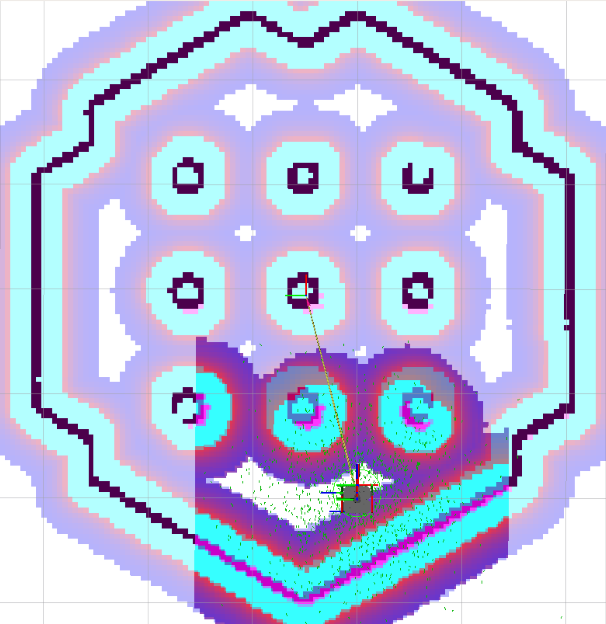
\includegraphics[width=8cm]{rviz.png}
    \centering
    \caption{Cost map displayed by RViz.}
    \label{fig:rviz}
\end{figure}

\filbreak

\subsection{Dijkstra's Algorithm} \label{dijkstra}
Dijkstra's algorithm is used to find the shortest path between two points in a network of nodes \parencite{computerphileDijkstraAlgorithmComputerphile2017}. As an example, consider the network shown in Figure \ref{fig:dijkstra}a. The goal is to find the shortest path from node A to node E. The following steps outline how to solve this problem using Dijkstra's algorithm.

\begin{figure}[htb]
    \centering
    \subfloat[\centering Shortest path is unknown] {{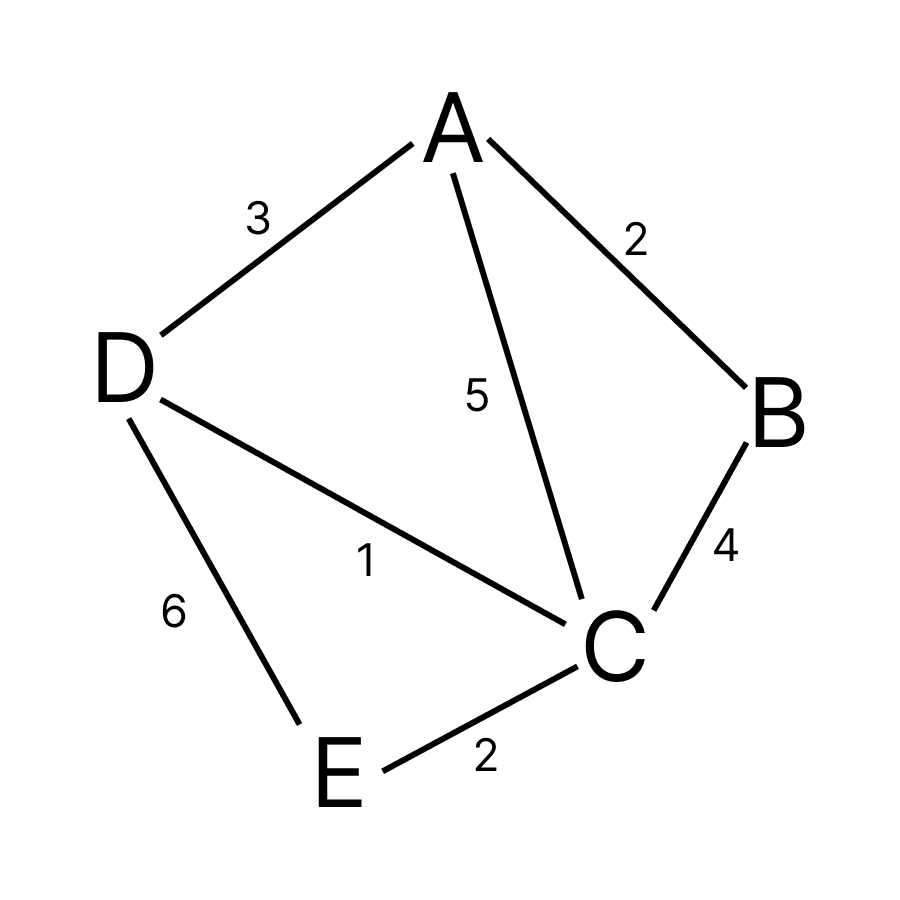
\includegraphics[width=5cm]{dijkstra1} }}
    \qquad
    \subfloat[\centering Shortest path is found]{{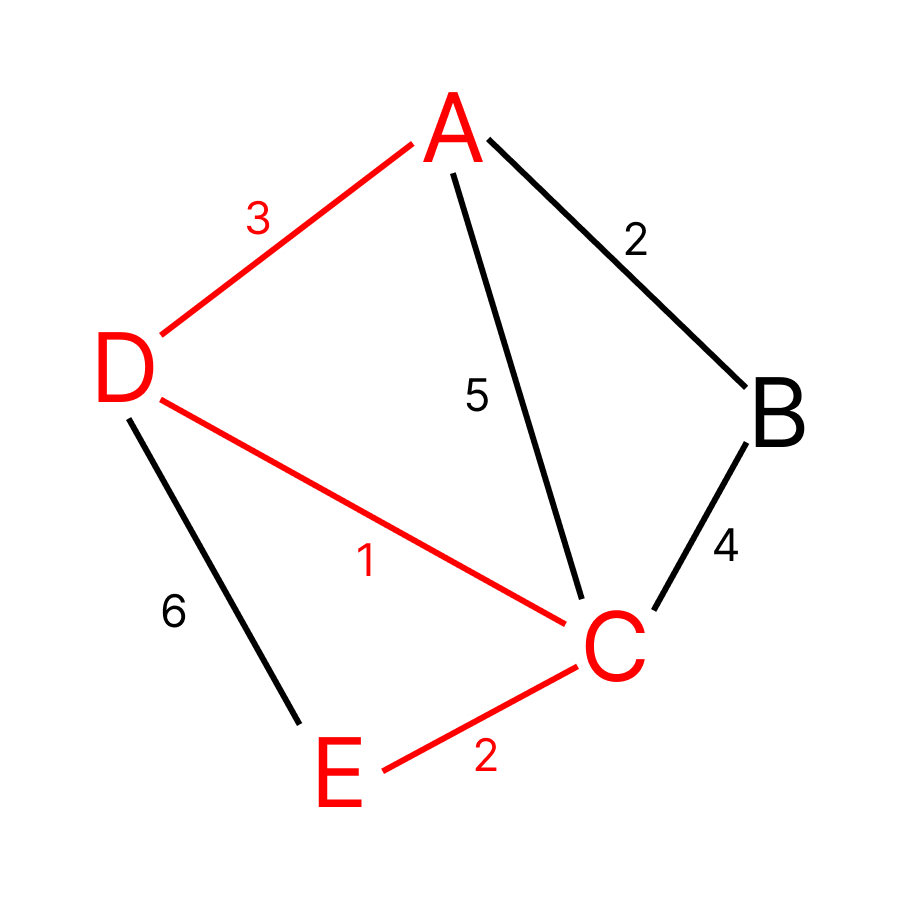
\includegraphics[width=5cm]{dijkstra2} }}
    \caption{Example of a network of nodes where the goal is to find the shortest path from node A to node E.}
    \label{fig:dijkstra}
\end{figure}

\begin{enumerate}
    \item \textbf{Current node: A}\\
          $\text{closed} = \{A\}$\\
          \def\arraystretch{1.5}
          \begin{tabular}{ |c|c|c|c|c|c|c|c| }
              \hline
                             & A & B & C & D & E        \\
              \hline
              Distance ($d$) & 0 & 2 & 5 & 3 & $\infty$ \\
              \hline
              Previous node  & - & A & A & A & A        \\
              \hline
          \end{tabular}
    \item \textbf{Current node: B}\\
          Since B is the closest node to A, it is added to the closed list.\\
          $\text{closed} = \{A,B\}$
          \begin{itemize}
              \item $d_C=\min(5,2+BC)=\min(5,2+4)=\min(5,6)=5$
              \item $d_D=\min(3,2+BD)=\min(3,2+\infty)=\min(3,\infty)=3$
              \item $d_E=\min(\infty,2+BE)=\min(\infty,2+\infty)=\min(\infty,\infty)=\infty$
          \end{itemize}
          Since there are no changes in the distance values, travelling from A to B directly is the shortest distance. Therefore, the previous nodes remain the same.
    \item \textbf{Current node: D}\\
          Node D is added to the closed list because it is the next the shortest path.\\
          $\text{closed} = \{A,B,D\}$
          \begin{itemize}
              \item $d_C=\min(5,3+DC)=\min(5,3+1)=\min(5,4)=4$
              \item $d_E=\min(\infty,3+DE)=\min(\infty,3+6)=\min(\infty,9)=9$
          \end{itemize}
          \def\arraystretch{1.5}
          \begin{tabular}{ |c|c|c|c|c|c|c|c| }
              \hline
                             & A & B & C & D & E \\
              \hline
              Distance ($d$) & 0 & 2 & 4 & 3 & 9 \\
              \hline
              Previous node  & - & A & D & A & D \\
              \hline
          \end{tabular}
    \item \textbf{Current node: C}\\
          Node C is added to the closed list because it has the shortest path from D.\\
          $\text{closed} = \{A,B,D,C\}$
          \begin{itemize}
              \item $d_E=\min(9,4+CE)=\min(9,4+2)=\min(9,6)=6$
          \end{itemize}
          \def\arraystretch{1.5}
          \begin{tabular}{ |c|c|c|c|c|c|c|c| }
              \hline
                             & A & B & C & D & E \\
              \hline
              Distance ($d$) & 0 & 2 & 4 & 3 & 6 \\
              \hline
              Previous node  & - & A & D & A & C \\
              \hline
          \end{tabular}
    \item It is possible to find the shortest path by working backwards from E ($E \leftarrow C \leftarrow D \leftarrow A$), as shown in Figure 4b. This path has a length of 6.
\end{enumerate}

\subsection{Global Path Planner} \label{global-planner}
In order for the robot to move towards a goal, a pathfinding algorithm is needed. In this project, the Navigation Function (NavFn) planner plugin from the Nav2 package is used \parencite{NavFnPlannerNav2}. To compute an optimal path to the goal, this plugin uses a potential field, called a navigation function. This field acts like a force that guides the robot's movement away from obstacles and towards the goal \parencite{philippsenInterpolatedDynamicNavigation2005}. It is represented by a grid map with each square having a discrete crossing time. As the navigation function is generated by propagating a wavefront outwards from the goal until it reaches the robot's starting position, the crossing time is the time at which the wavefront crosses a grid square. The wavefront's position at a time $t$ is given by
\[
    \Gamma (t)=\{(x,y) \mid T(x,y)=t\}.
\]

The potential field is built from the cost map described in section \ref{cost-map}. The costs on the cost map are converted to wavefront propagation speeds ($F$) \parencite{philippsenInterpolatedDynamicNavigation2005}. A lower cost is converted to a higher speed, while a higher cost is converted to a lower speed. If $F(x,y)>0$, the navigation function follows the differential equation
\[
    |\nabla T|F=1.
\]
As the navigation function is represented by a discrete grid map, this equation needs to be written in a discrete notation. For a given square located at ($i,j$), its crossing time ($T$) can be found using the equation
\[
    \max(D_{ij}^{-x}T,-D_{ij}^{+x},0)^2+\max(D_{ij}^{-y}T,-D_{ij}^{+y},0)^2=\frac{1}{F_{ij}^2}.
\]





\parencite{macenskiDesksROSMaintainers2023}

% From the cost map, the algorithm converts the cost of each square to a wavefront speed.

% The potential field is represented by a grid map with each square having a discrete crossing time, as shown in Figure \ref{fig:potential}.  Thus, Dijkstra's algorithm uses this wavefront speed to find the smallest crossing time for a cell.

A minimum travel cost is used so that the cost increases as the field propagates further. Hence, the goal is the navigation function's only minimum and the optimal path can be found using gradient descent, an iterative minimization algorithm \parencite{GradientDescent2024}. Gradient descent works by taking ``repeated steps in the opposite direction of the gradient'' \parencite{GradientDescent2024}.


"where $F_{ij}$ is the known propagation speed at cell (i,j)" and the $D_{ij}$ terms are the Newton quotients along their respective axes.

\begin{figure}[htb]
    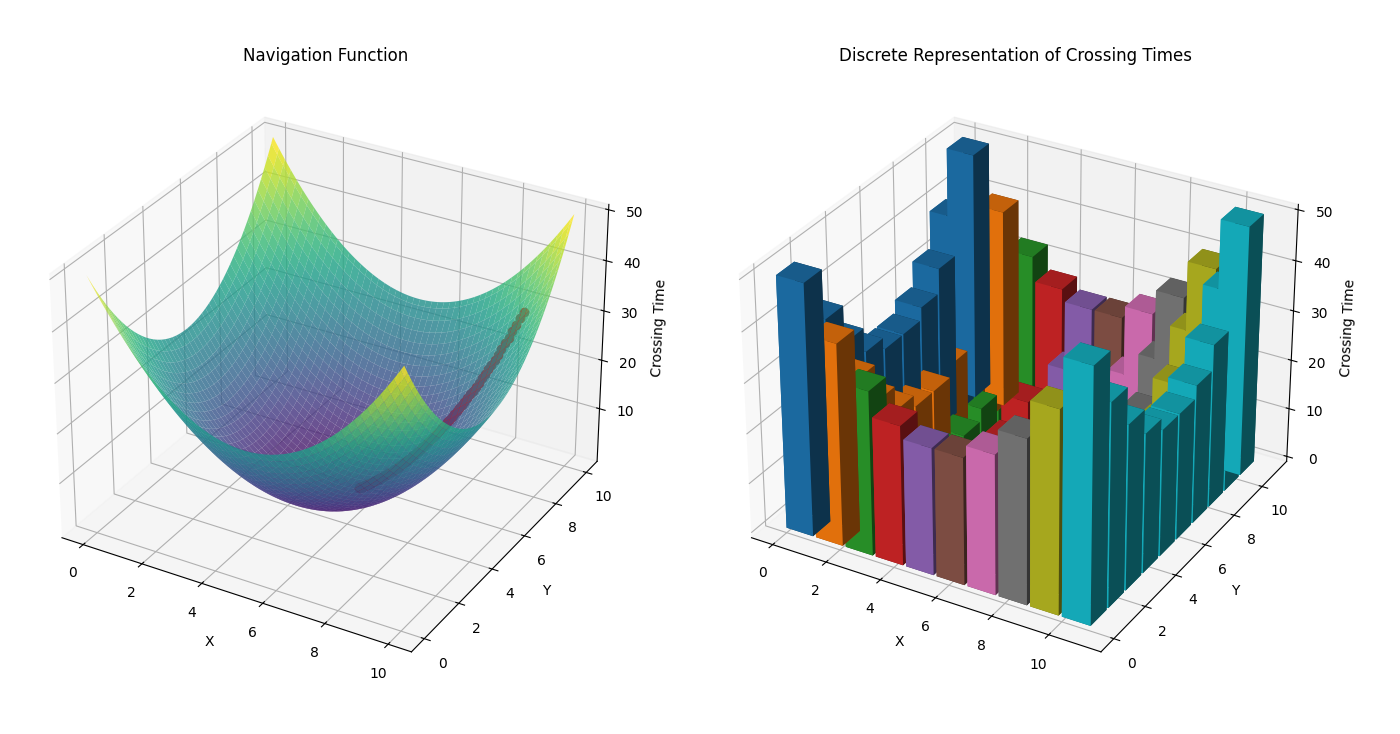
\includegraphics[width=12cm]{potential.png}
    \centering
    \caption{3D representation of how the continuous navigation function is discretized into a crossing time for each square on the map. The red line denotes the path of the robot towards the goal.}
    \label{fig:potential}
\end{figure}